\chapter{Neuronas, potenciales de acción y sinapsis}\label{ch:b2:neurons-synapses}

Si se golpea el tendón situado bajo la rótula, la pierna da una patada
treinta milisegundos después. En ese tiempo se ha detectado un
estiramiento en el muslo, una señal ha recorrido un metro hasta la médula
espinal, ha cruzado una unión hacia una segunda célula, ha recorrido un
metro de vuelta y ha hecho contraerse un músculo --- todo el trayecto de
ida y vuelta más rápido que un parpadeo. Ninguna \omterm{def:b2:cell-signalling:kinds}{hormona} podría hacerlo;
lo hacen células construidas para conducir, y una señal que no es una
sustancia en movimiento sino una onda eléctrica que se regenera a lo largo
de una membrana. Este capítulo trata de esa célula y de esa señal: el
voltaje que una \omterm{def:b2:neurons-synapses:neuron}{neurona} mantiene a través de su membrana, el impulso que
emite y cómo se propaga, y la \omterm{def:b2:neurons-synapses:synapse}{sinapsis}, donde la señal eléctrica se
convierte en química y vuelve a hacerse eléctrica.

\section{La neurona}

\begin{definition}[Neurona, axón, nervio]\label{def:b2:neurons-synapses:neuron}
\index{neurona}\index{axón}\index{dendrita}\index{mielina}\index{glía}
Una \emph{neurona} es una célula especializada en la señalización: un
cuerpo celular (\emph{soma}) con el núcleo, unas \emph{dendritas}
ramificadas que reciben las señales y un único \emph{axón} --- un cable
de uno a veinte micrómetros de grosor y de hasta un metro de longitud ---
que lleva su salida hasta unas \emph{terminales} situadas sobre otras
células. El encéfalo humano tiene unas $10^{11}$ neuronas, y cada una
forma alrededor de mil \omterm{def:b2:neurons-synapses:synapse}{sinapsis}. Las neuronas son menos numerosas que
las células de la \emph{glía}: los astrocitos, que las alimentan y
amortiguan su entorno; la microglía, que las vigila; y las células que
envuelven los axones con \emph{mielina} --- decenas de vueltas de su
propia membrana, casi sin citoplasma, que forman una vaina aislante
interrumpida más o menos cada milímetro en los \emph{\omterm{prop:b2:neurons-synapses:myelin}{nódulos de Ranvier}}.
Un \emph{nervio} es un haz de miles de axones, sensitivos y motores, que
discurren juntos en un tejido conjuntivo. Las neuronas no se dividen en
el adulto (con pocas excepciones), y un axón separado de su cuerpo celular
muere; una neurona es una célula que debe durar toda una vida.
\end{definition}
\begin{omfigure}
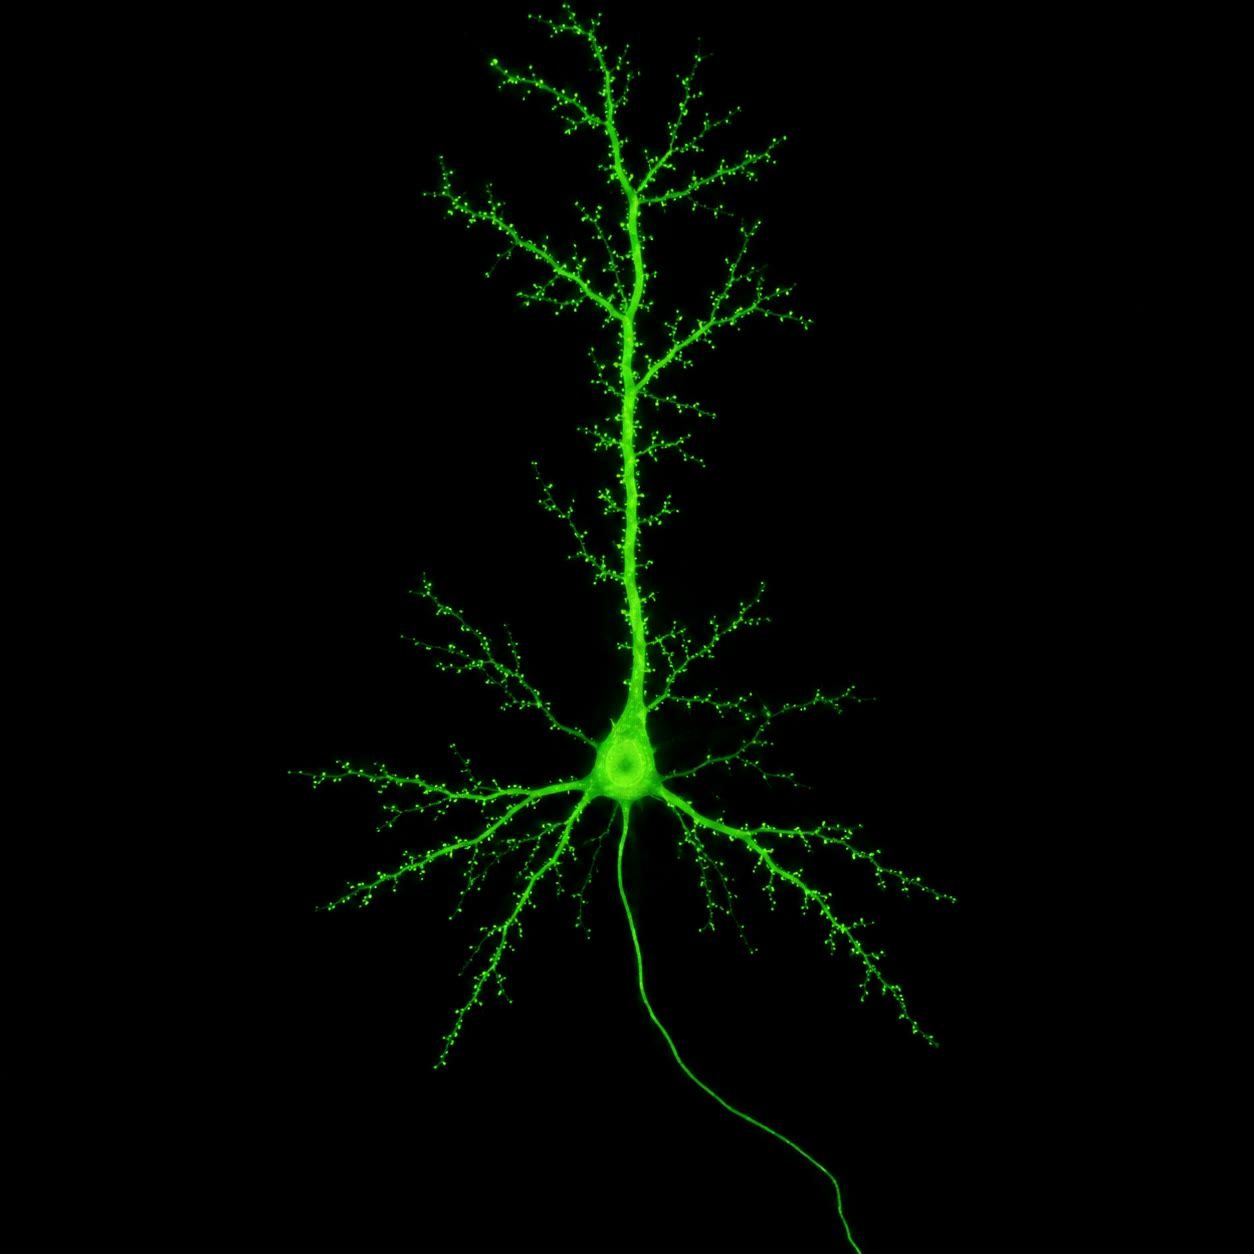
\includegraphics[width=0.4\linewidth]{images/book4/ai/b4-20-neuron-fluorescence.jpg}\hspace{0.05\linewidth}
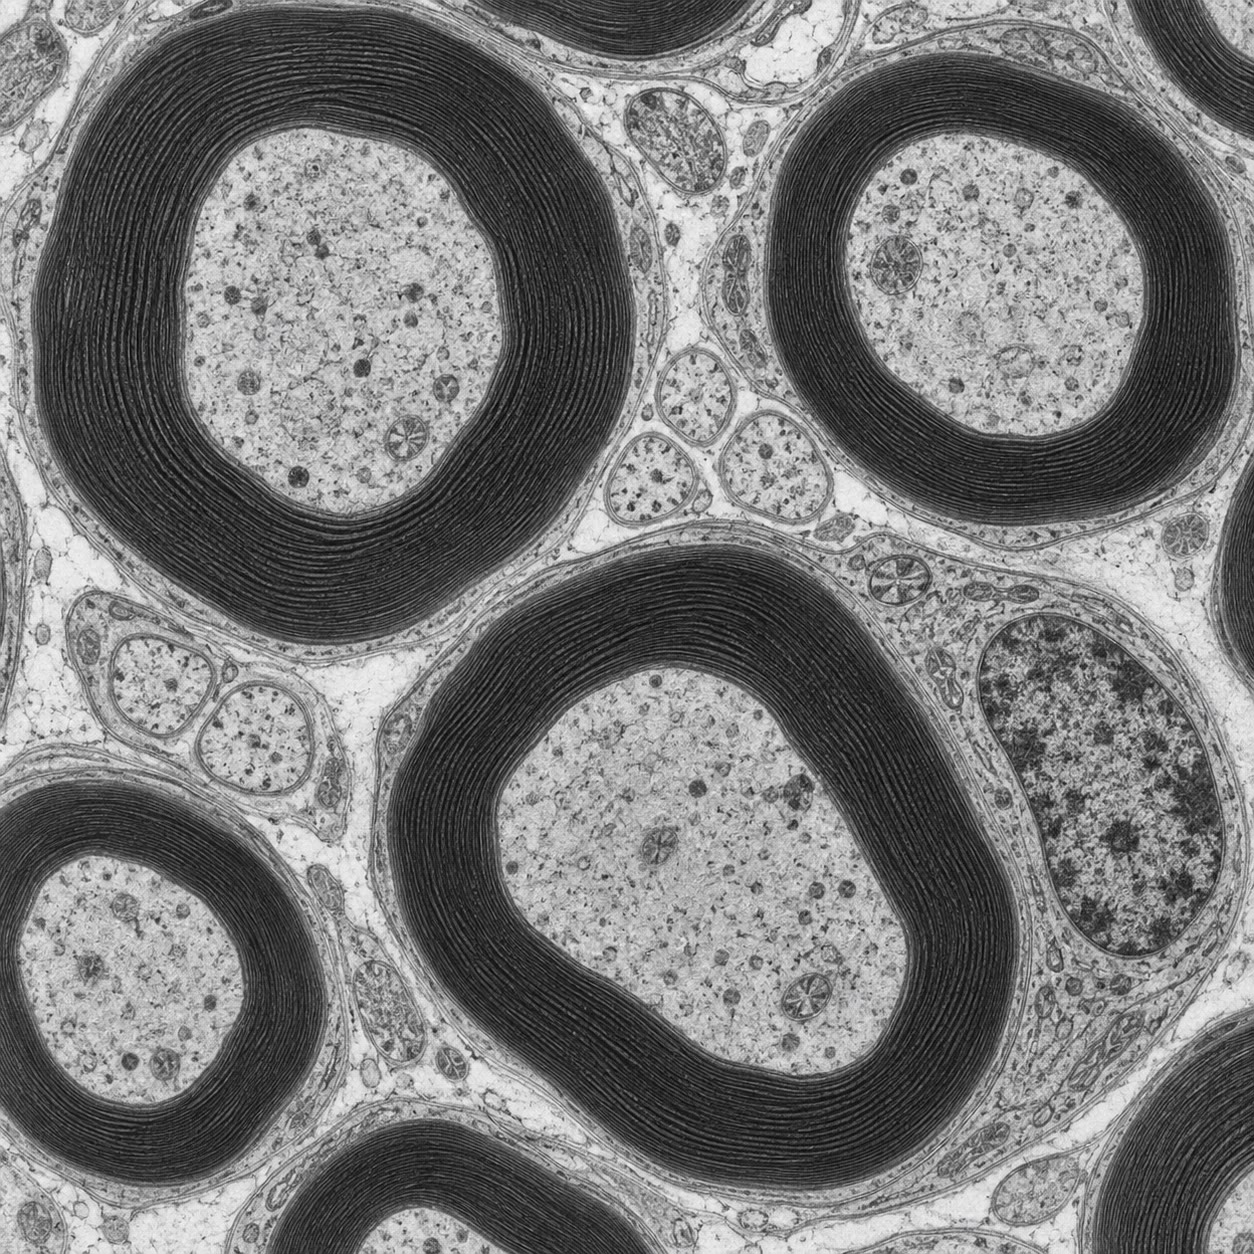
\includegraphics[width=0.4\linewidth]{images/book4/ai/b4-20-myelinated-axons-tem.jpg}

{\small Izquierda: una \omterm{def:b2:neurons-synapses:neuron}{neurona} piramidal rellena de colorante --- el
cuerpo celular, las \omterm{def:b2:neurons-synapses:neuron}{dendritas} espinosas que reciben y el fino \omterm{def:b2:neurons-synapses:neuron}{axón} que sale
de la base. Derecha: \omterm{def:b2:neurons-synapses:neuron}{axones} en sección transversal al microscopio
electrónico, cada uno envuelto en la espiral oscura de su vaina de \omterm{def:b2:neurons-synapses:neuron}{mielina}.}
\end{omfigure}

\section{El potencial de reposo}

\begin{theorem}[El potencial de Nernst]\label{thm:b2:neurons-synapses:nernst}
\index{potencial de Nernst}\index{potencial de equilibrio}
Una membrana permeable a un solo ion de carga $z$, que separa las
concentraciones $c_{\text{ext}}$ y $c_{\text{int}}$, se estabiliza en el
\emph{\omterm{thm:b2:neurons-synapses:nernst}{potencial de equilibrio}}, en el que la fuerza eléctrica sobre el ion
compensa su difusión:
\[
E = \frac{RT}{zF}\ln\frac{c_{\text{ext}}}{c_{\text{int}}} \approx \frac{\qty{61.5}{mV}}{z}\log_{10}\frac{c_{\text{ext}}}{c_{\text{int}}} \quad (\qty{37}{\celsius}).
\]
Una \omterm{def:b2:neurons-synapses:neuron}{neurona} mantiene \qty{140}{mmol/L} de potasio en el interior frente
a \qty{5}{mmol/L} en el exterior, y \qty{15}{mmol/L} de sodio en el
interior frente a \qty{145}{mmol/L} en el exterior, gradientes creados
por la bomba de sodio--potasio a costa de un tercio del ATP de la célula.
De ahí que $E_{\mathrm K} = 61.5\log_{10}(5/140) = \qty{-89}{mV}$ y
$E_{\mathrm{Na}} = 61.5\log_{10}(145/15) = \qty{+61}{mV}$: si la
membrana solo dejara pasar potasio, se situaría en
\qty{-89}{mV}; si solo dejara pasar sodio, en \qty{+61}{mV}.
\end{theorem}
\begin{proof}
En el equilibrio, el potencial electroquímico del ion es el mismo a ambos
lados: $RT\ln c_{\text{int}} + zFV_{\text{int}} = RT\ln
c_{\text{ext}} + zFV_{\text{ext}}$, de modo que $V_{\text{int}} -
V_{\text{ext}} = (RT/zF)\ln(c_{\text{ext}}/c_{\text{int}})$. A
\qty{310}{K}, $RT/F = \qty{26.7}{mV}$ y $\ln 10 \times 26.7 =
\qty{61.5}{mV}$. (Deducido en el volumen del primer año a partir de la
distribución de Boltzmann; aquí solo se recuerda.)
\end{proof}

\begin{theorem}[El potencial de reposo como media ponderada]\label{thm:b2:neurons-synapses:chord}
\index{potencial de reposo}\index{conductancia (membrana)}
Si la membrana conduce varios iones, cada uno con una conductancia $g_i$
(la facilidad con que lo deja pasar, fijada por el número de canales
abiertos), el potencial estacionario en el que las corrientes se anulan es
\[
V = \frac{\sum_i g_i E_i}{\sum_i g_i},
\]
una media de los \omterm{thm:b2:neurons-synapses:nernst}{potenciales de equilibrio} ponderada por las
conductancias. En reposo, la membrana de una \omterm{def:b2:neurons-synapses:neuron}{neurona} es unas veinte veces
más permeable al potasio que al sodio, de modo que $V \approx (20\times(-89) +
61)/21 = \qty{-82}{mV}$; si se cuentan el cloruro y las pequeñas fugas, el
\omterm{thm:b2:neurons-synapses:chord}{potencial de reposo} es de \qty{-70}{mV}. La membrana reposa cerca de
$E_{\mathrm K}$ porque los canales de potasio están abiertos; todo lo que
abre canales de sodio la arrastra hacia $E_{\mathrm{Na}}$ --- y en eso
consiste todo el principio de la señalización nerviosa.
\end{theorem}
\begin{proof}
Cada ion transporta una corriente $I_i = g_i(V - E_i)$ (ley de Ohm, con la
fuerza impulsora medida desde el propio equilibrio del ion). Con un
potencial estacionario, la corriente total es nula: $\sum_i g_i(V - E_i) =
0$, de donde $V\sum g_i = \sum g_iE_i$. (El tratamiento completo, en el
que las permeabilidades intervienen mediante la ecuación de
Goldman--Hodgkin--Katz, da la misma ponderación en primer orden.)
\end{proof}
\section{El potencial de acción}

\begin{proposition}[El impulso]\label{prop:b2:neurons-synapses:ap}
\index{potencial de acción}\index{canal dependiente de voltaje}\index{umbral}\index{periodo refractario}
La membrana del \omterm{def:b2:neurons-synapses:neuron}{axón} contiene \emph{canales de sodio dependientes de
voltaje}, cerrados en reposo y abiertos por la despolarización. Si un
estímulo eleva el potencial desde \qty{-70}{mV} por encima de un
\emph{umbral} cercano a \qty{-55}{mV}, se abren suficientes canales para
dejar entrar más sodio del que puede compensar la fuga de potasio; el
potencial sube, se abren más canales y, en una fracción de milisegundo,
la membrana es arrastrada hacia
$E_{\mathrm{Na}}$ --- una \emph{retroalimentación positiva} explosiva y
de todo o nada. Alcanza su máximo cerca de \qty{+40}{mV} porque los
canales de sodio se \emph{inactivan} en el milisegundo que sigue a su
apertura y porque unos \emph{canales de potasio dependientes de voltaje}
más lentos se abren y devuelven el potencial hacia $E_{\mathrm K}$,
sobrepasándolo hasta una \emph{hiperpolarización posterior} antes de que
se cierren los canales de potasio. El \emph{\omterm{prop:b2:neurons-synapses:ap}{potencial de acción}} dura
alrededor de un milisegundo; durante otro milisegundo o dos, los canales
de sodio inactivados no pueden volver a abrirse (el \emph{\omterm{prop:b2:neurons-synapses:ap}{periodo
refractario}}), lo que limita la frecuencia de disparo a unos cientos por
segundo y obliga al impulso a propagarse en un solo sentido. Como es de
todo o nada, el impulso no transporta información en su tamaño: la
\omterm{def:b2:neurons-synapses:neuron}{neurona} codifica la intensidad en su \emph{frecuencia}. Unos
$10^{4}$ iones de sodio entran y otros tantos iones de potasio salen en
cada impulso --- un cambio de concentración despreciable, que la bomba
restablece sin prisa.
\end{proposition}
\begin{proof}[Evidencia]
Hodgkin y Huxley (1952), con el \omterm{def:b2:neurons-synapses:neuron}{axón} gigante del calamar (de medio
milímetro de grosor, lo que permitía introducir un hilo en su interior) y
un amplificador de retroalimentación que mantenía el potencial de membrana
en cualquier valor elegido (la \emph{fijación de voltaje}) mientras
registraba la corriente necesaria para mantenerlo, separaron la corriente
en un componente precoz entrante, que desaparecía al retirar el sodio del
baño, y un componente tardío saliente, transportado por el potasio;
midieron cómo subía y bajaba cada conductancia con el tiempo a cada
voltaje; y, ajustando cada una con unas pocas ecuaciones, calcularon la
forma, el umbral, la velocidad y el \omterm{prop:b2:neurons-synapses:ap}{periodo refractario} del \omterm{prop:b2:neurons-synapses:ap}{potencial de
acción} a partir de las dos conductancias solas. Todas las predicciones se
cumplieron. Los propios canales se observaron veinticinco años más tarde,
uno a uno, registrando pequeños fragmentos de membrana; la tetrodotoxina
(el veneno del pez globo) bloquea el canal de sodio y suprime el impulso,
y el tetraetilamonio bloquea el canal de potasio y lo prolonga.
\end{proof}
\begin{omfigure}
\begin{tikzpicture}
\begin{axis}[
  width=0.9\linewidth, height=6.4cm,
  axis x line=bottom, axis y line=left,
  xmin=0, xmax=4, ymin=-100, ymax=60,
  xlabel={tiempo (ms)}, ylabel={potencial de membrana (mV)},
  xlabel style={font=\small, at={(axis description cs:0.5,-0.1)}, anchor=north},
  ylabel style={font=\small},
  tick label style={font=\small}, xtick={0,1,2,3,4}, ytick={-90,-70,-55,0,40},
  legend style={font=\scriptsize, at={(0.97,0.95)}, anchor=north east, draw=none},
  clip=false,
]
\addplot[very thick, omDef] coordinates {(0,-70) (0.4,-70) (0.5,-64) (0.6,-55) (0.7,-30) (0.8,10) (0.9,35) (1.0,40) (1.1,30) (1.2,10) (1.35,-20) (1.5,-50) (1.7,-75) (1.9,-85) (2.2,-82) (2.6,-76) (3.2,-71) (4,-70)};
\addlegendentry{potencial de membrana}
\addplot[thick, omThm, dashed] coordinates {(0,0) (0.5,0) (0.6,5) (0.7,20) (0.8,35) (0.9,30) (1.0,20) (1.1,8) (1.2,3) (1.4,0) (4,0)};
\addlegendentry{$g_{\mathrm{Na}}$ (relativa)}
\addplot[thick, omProp, dashed] coordinates {(0,0) (0.6,0) (0.8,2) (1.0,8) (1.2,16) (1.4,20) (1.7,17) (2.0,10) (2.4,4) (3.0,1) (4,0)};
\addlegendentry{$g_{\mathrm K}$ (relativa)}
\draw[dashed, gray] (axis cs:0,-55) -- (axis cs:4,-55); \node[font=\scriptsize, anchor=south east] at (axis cs:4,-55) {umbral};
\draw[dashed, gray] (axis cs:0,-89) -- (axis cs:4,-89); \node[font=\scriptsize, anchor=south east] at (axis cs:3.7,-89) {$E_{\mathrm K}$};
\draw[<->, gray] (axis cs:1.0,50) -- (axis cs:2.5,50); \node[font=\scriptsize, anchor=south, gray] at (axis cs:1.75,50) {refractario};
\end{axis}
\end{tikzpicture}

{\small Un \omterm{prop:b2:neurons-synapses:ap}{potencial de acción}. Superado el umbral, la conductancia al
sodio (en rojo) sube de forma explosiva y arrastra el potencial hacia
$E_{\mathrm{Na}}$; se inactiva mientras la conductancia al potasio
(en naranja) sube y devuelve la membrana hacia $E_{\mathrm K}$, con una
hiperpolarización posterior. Por debajo de la línea del umbral, no ocurre
nada.}
\end{omfigure}

\section{La conducción}

\begin{theorem}[El cable y su constante de longitud]\label{thm:b2:neurons-synapses:cable}
\index{constante de longitud}\index{ecuación del cable}\index{velocidad de conducción}
Un \omterm{def:b2:neurons-synapses:neuron}{axón} es un cable con fugas: la corriente inyectada en un punto fluye a
lo largo del citoplasma (resistencia $r_i$ por unidad de longitud) y se
escapa a través de la membrana (resistencia $r_m$ por unidad de
longitud). Una despolarización estacionaria $V_0$ en $x = 0$ decae a lo
largo del \omterm{def:b2:neurons-synapses:neuron}{axón} como
\[
V(x) = V_0\,e^{-x/\lambda}, \qquad \lambda = \sqrt{\frac{r_m}{r_i}} = \sqrt{\frac{R_m\,d}{4R_i}},
\]
donde $d$ es el diámetro y $R_m$, $R_i$ las resistencias específicas de la
membrana y del citoplasma. La \emph{\omterm{thm:b2:neurons-synapses:cable}{constante de longitud}}
$\lambda$ es la distancia a lo largo de la cual una señal pasiva cae a
un tercio: unos \qty{0.5}{mm} para un \omterm{def:b2:neurons-synapses:neuron}{axón} de \qty{1}{\micro m}, y crece
como la raíz cuadrada del diámetro. Un \omterm{prop:b2:neurons-synapses:ap}{potencial de acción} se propaga
porque la despolarización de su frente, que se extiende pasivamente por
delante a lo largo de unos $\lambda$, lleva el tramo siguiente de membrana
al umbral, y este la regenera a tamaño completo; cuanto más lejos llega,
más rápida es la onda, de modo que la \omterm{thm:b2:neurons-synapses:cable}{velocidad de conducción} también
crece aproximadamente como $\sqrt{d}$ --- desde \qty{1}{m/s} en una fibra
fina amielínica hasta \qty{20}{m/s} en el \omterm{def:b2:neurons-synapses:neuron}{axón} gigante del calamar.
\end{theorem}
\begin{proof}
Sean $i(x)$ la corriente axial y $V(x)$ la despolarización de la
membrana. La ley de Ohm a lo largo del axoplasma da $\mathrm{d}V/
\mathrm{d}x = -r_i\,i$; la conservación de la carga, con la fuga a través
de la membrana, da $\mathrm{d}i/\mathrm{d}x = -V/r_m$. Combinándolas,
$\mathrm{d}^{2}V/\mathrm{d}x^{2} = V/(r_m r_i)$, cuya solución
decreciente es $V_0 e^{-x/\lambda}$ con $\lambda^{2} = r_m/r_i$. Para un
cilindro, $r_m = R_m/(\pi d)$ y $r_i = 4R_i/(\pi d^{2})$, de modo que
$\lambda^{2} = R_m d/4R_i$. Con $R_m = \qty{1}{\ohm.m^2}$, $R_i =
\qty{1}{\ohm.m}$ y $d = \qty{1}{\micro m}$: $\lambda = \sqrt{10^{-6}
/4} = \qty{0.5}{mm}$.
\end{proof}

\begin{proposition}[La mielina y la conducción saltatoria]\label{prop:b2:neurons-synapses:myelin}
\index{conducción saltatoria}\index{nódulo de Ranvier}
La \omterm{def:b2:neurons-synapses:neuron}{mielina} multiplica $r_m$ por el número de vueltas de membrana y divide
la capacidad de la membrana por el mismo factor, de modo que bajo la vaina
casi no se escapa corriente y hace falta poca carga para cambiar el
potencial: la despolarización se extiende pasivamente a lo largo de un
internodo de un milímetro con pocas pérdidas, y el \omterm{prop:b2:neurons-synapses:ap}{potencial de acción}
solo se regenera en los nódulos, donde se concentran los canales de sodio.
Así, el impulso \emph{salta} de nódulo en nódulo
(\emph{\omterm{prop:b2:neurons-synapses:myelin}{conducción saltatoria}}), a \qty{100}{m/s} en una fibra de
\qty{20}{\micro m} --- una velocidad que un \omterm{def:b2:neurons-synapses:neuron}{axón} amielínico solo
alcanzaría con centímetros de grosor --- y con una fracción del coste
metabólico, puesto que el sodio solo entra en los nódulos. La \omterm{def:b2:neurons-synapses:neuron}{mielina} es
la invención de los vertebrados que hizo posible un sistema nervioso
grande y rápido en un cuerpo pequeño; en la esclerosis múltiple, la vaina
se destruye a parches, la \omterm{thm:b2:neurons-synapses:cable}{constante de longitud} se desploma y los
impulsos fallan.
\end{proposition}
\begin{omfigure}
\begin{tikzpicture}[every node/.style={font=\scriptsize}, >=stealth]
  % unmyelinated
  \begin{scope}
    \draw[thick, fill=omDef!10] (0,0) rectangle (11,0.5);
    \foreach \x in {0.5,1.0,...,10.5} \draw[omThm, ->] (\x,0.25) -- (\x,0.9);
    \node[anchor=east] at (-0.2,0.25) {amielínico};
    \node[anchor=west] at (11.2,0.25) {\qty{1}{m/s}};
    \node[above] at (5.5,1.0) {el impulso se regenera en cada punto};
  \end{scope}
  % myelinated
  \begin{scope}[yshift=-2.4cm]
    \draw[thick, fill=omDef!10] (0,0) rectangle (11,0.5);
    \foreach \x in {0.3,2.5,4.7,6.9,9.1} \fill[omExo!60] (\x,-0.15) rectangle (\x+1.9,0.65);
    \foreach \x in {2.35,4.55,6.75,8.95} \draw[omThm, ->] (\x,0.25) -- (\x,0.9);
    \foreach \x in {2.35,4.55,6.75} \draw[->, thick, omThm, dashed] (\x+0.1,1.1) .. controls (\x+1.1,1.6) .. (\x+2.1,1.1);
    \node[anchor=east] at (-0.2,0.25) {mielínico};
    \node[anchor=west] at (11.2,0.25) {\qty{100}{m/s}};
    \node[below] at (1.25,-0.2) {internodo de mielina};
    \node[below] at (4.55,-0.2) {nódulo de Ranvier};
    \node[above] at (5.5,1.6) {regenerado solo en los nódulos: saltatoria};
  \end{scope}
\end{tikzpicture}

{\small La conducción con y sin \omterm{def:b2:neurons-synapses:neuron}{mielina}. En un \omterm{def:b2:neurons-synapses:neuron}{axón} desnudo, el impulso se
regenera a todo lo largo; bajo la \omterm{def:b2:neurons-synapses:neuron}{mielina}, la señal se extiende pasivamente
por cada internodo y se regenera en los nódulos, y el impulso viaja cien
veces más deprisa.}
\end{omfigure}

\section{La sinapsis}

\begin{definition}[Sinapsis químicas y eléctricas]\label{def:b2:neurons-synapses:synapse}
\index{sinapsis}\index{neurotransmisor}\index{potencial postsináptico}
En una \emph{sinapsis}, la terminal de una \omterm{def:b2:neurons-synapses:neuron}{neurona} se encuentra con una
diana --- otra \omterm{def:b2:neurons-synapses:neuron}{neurona}, una \omterm{def:b2:cell-differentiation:myogenesis}{fibra muscular}, una célula glandular. En una
sinapsis \emph{eléctrica}, uniones comunicantes conectan las dos células y
la corriente pasa directamente --- rápida, bidireccional, sin
amplificación, empleada donde importan la velocidad y la sincronía
(reflejos de huida, el \omterm{def:b2:heart:anatomy}{corazón}). En una sinapsis \emph{química}, las
células están separadas por una hendidura de \qty{20}{nm} y la señal es
una molécula. Un \omterm{prop:b2:neurons-synapses:ap}{potencial de acción} que llega a la terminal abre canales
de calcio dependientes de voltaje; el calcio entra y, en una fracción de
milisegundo, hace que vesículas de \emph{neurotransmisor} se fusionen con
la membrana y se vacíen en la hendidura; el transmisor la atraviesa por
difusión en microsegundos y se une a receptores de la membrana
postsináptica --- ya sean canales iónicos que abre (\emph{ionotrópicos},
rápidos) o \omterm{prop:b2:cell-signalling:gpcr}{receptores acoplados a proteínas G}
(\emph{metabotrópicos}, más lentos, \cref{ch:b2:cell-signalling}); la
corriente resultante desplaza el potencial postsináptico unos pocos
milivoltios, hacia arriba (un \emph{potencial postsináptico excitador},
debido a canales que dejan pasar sodio) o hacia abajo (uno
\emph{inhibidor}, debido a canales que dejan pasar cloruro o potasio); y
el transmisor se retira en milisegundos mediante una enzima o un
transportador. El retraso es de medio milisegundo; ese precio compra la
transmisión en un solo sentido, la amplificación, la inhibición y la
modificabilidad --- todo lo que un sistema nervioso necesita más allá de
la mera conducción.
\end{definition}
\begin{omfigure}
\begin{tikzpicture}[every node/.style={font=\scriptsize}, >=stealth]
  % presynaptic terminal
  \draw[thick, fill=omDef!10] (0,0) .. controls (0,2.6) and (3.6,2.6) .. (3.6,0.2) -- (3.6,-0.2) .. controls (3.6,-2.6) and (0,-2.6) .. (0,0);
  \draw[very thick, omDef] (-2.2,0) -- (0.1,0); \node[omDef, above] at (-1.1,0.05) {axón};
  \foreach \p in {(2.0,1.0),(2.6,0.5),(2.7,-0.4),(2.1,-1.0),(1.6,0.2)} \draw[thick, fill=omProp!40] \p circle (0.25);
  \draw[thick, fill=omProp!40] (3.3,0.1) arc (90:-90:0.25) -- cycle;
  \foreach \p in {(3.75,0.2),(3.85,-0.1),(3.7,-0.35),(3.9,0.4)} \fill[omProp] \p circle (0.05);
  \fill[omThm] (3.45,1.3) circle (0.06); \node[omThm, anchor=east] at (3.35,1.45) {entra Ca$^{2+}$};
  \draw[->, omThm] (3.9,1.5) -- (3.55,1.35);
  % cleft
  \node[align=center, anchor=north] at (3.85,-2.75) {hendidura\\\qty{20}{nm}};
  \draw[gray] (3.85,-2.7) -- (3.85,-1.2);
  % postsynaptic
  \draw[thick, fill=omExo!15] (4.1,-2.6) rectangle (8.2,2.6);
  \foreach \y in {0.9,0.3,-0.3,-0.9} \draw[thick, fill=omDef!40] (4.05,\y-0.15) rectangle (4.45,\y+0.15);
  \node[anchor=west, align=left] at (4.6,0.3) {receptores: canales\\abiertos, flujo\\de iones, potencial\\postsináptico};
  \node[anchor=west, align=left] at (4.6,-1.7) {transmisor retirado\\por una enzima o\\un transportador};
  \node[anchor=west] at (4.6,2.2) {célula postsináptica};
  % labels
  \node[align=center, anchor=north] at (1.8,-2.75) {vesículas de\\transmisor};
  \node[anchor=south] at (1.8,2.75) {terminal presináptica};
\end{tikzpicture}

{\small Una \omterm{def:b2:neurons-synapses:synapse}{sinapsis} química. El impulso deja entrar calcio, las vesículas
se fusionan y liberan el transmisor en la hendidura, los receptores de la
diana abren canales y el transmisor se elimina en milisegundos.}
\end{omfigure}

\begin{theorem}[Liberación cuántica]\label{thm:b2:neurons-synapses:quantal}
\index{liberación cuántica}\index{potencial miniatura}
El transmisor se libera en paquetes --- \emph{cuantos}, de una vesícula
cada uno ---, y el número $k$ liberado por un impulso es una variable
aleatoria. Si la terminal posee $n$ sitios de liberación que liberan cada
uno con probabilidad $p$, y $p$ es pequeña, $k$ sigue aproximadamente una
ley de Poisson de media $m = np$:
\[
P(k) = \frac{m^{k}e^{-m}}{k!}, \qquad P(0) = e^{-m}, \qquad
m = \ln\frac{\text{número de ensayos}}{\text{número de fallos}}.
\]
El contenido cuántico medio $m$ puede leerse, por tanto, a partir de la
fracción de impulsos que no liberan nada, y comprobarse frente a la
respuesta media dividida por el tamaño de un cuanto. En una \omterm{prop:b2:neurons-synapses:integration}{unión
neuromuscular}, $m$ es de unos cientos --- la transmisión nunca falla; en
una \omterm{def:b2:neurons-synapses:synapse}{sinapsis} central suele estar cerca de uno, y la \omterm{def:b2:neurons-synapses:synapse}{sinapsis} solo
transmite una fracción de los impulsos.
\end{theorem}
\begin{proof}
Con $n$ sitios independientes que liberan cada uno con probabilidad $p$, $k$
es binomial; para $n$ grande y $p$ pequeña con $np = m$ fija, la binomial
tiende a la ley de Poisson (serie de matemáticas, segundo año).
$P(0) = e^{-m}$ da $m$ a partir de los fallos. La comprobación de Katz
consiste en que la misma $m$, introducida en la fórmula de Poisson,
predice las fracciones observadas de respuestas de uno, dos y tres cuantos.
\end{proof}
\begin{proof}[Evidencia]
Fatt y Katz (1952) registraron en una \omterm{def:b2:cell-differentiation:myogenesis}{fibra muscular} de rana en reposo
pequeñas despolarizaciones espontáneas de unos \qty{0.5}{mV}, todas del
mismo tamaño, a intervalos aleatorios --- los \emph{potenciales de placa
terminal en miniatura}, cada uno debido a una vesícula. Al reducir el
calcio del baño, la respuesta a la estimulación del nervio disminuía hasta
fluctuar entre 0, 1, 2 o 3 múltiplos del tamaño miniatura; las
frecuencias de los múltiplos seguían la ley de Poisson con la
$m$ calculada a partir de los fallos. Del Castillo y Katz demostraron así
que la liberación es cuántica y que el calcio controla la probabilidad de
liberación y no el tamaño de un cuanto, y la microscopía electrónica
mostró las vesículas que constituyen los cuantos.
\end{proof}

\begin{proposition}[Integración: la neurona como decisión]\label{prop:b2:neurons-synapses:integration}
\index{sumación}\index{cono axónico}\index{unión neuromuscular}
Una \omterm{def:b2:neurons-synapses:neuron}{neurona} central recibe miles de \omterm{def:b2:neurons-synapses:synapse}{sinapsis}, excitadoras e inhibidoras,
en sus \omterm{def:b2:neurons-synapses:neuron}{dendritas} y su soma. Cada \omterm{def:b2:neurons-synapses:synapse}{potencial postsináptico} es pequeño y
decae pasivamente, con la \omterm{thm:b2:neurons-synapses:cable}{constante de longitud} del cable en el espacio y
la constante de tiempo de la membrana (unos pocos milisegundos) en el
tiempo; se suman --- \emph{sumación espacial} de las entradas que llegan
juntas, \emph{sumación temporal} de las entradas que llegan en rápida
sucesión --- y la suma se lee en el \emph{\omterm{prop:b2:neurons-synapses:integration}{cono axónico}}, donde los
canales de sodio son más densos y el umbral más bajo. Si la suma supera el
umbral, el \omterm{def:b2:neurons-synapses:neuron}{axón} dispara, a una frecuencia que crece con el exceso; las
entradas inhibidoras restan, y una \omterm{def:b2:neurons-synapses:synapse}{sinapsis} inhibidora próxima al cono
puede vetar una excitadora lejana. La
\omterm{prop:b2:neurons-synapses:integration}{unión neuromuscular} es la excepción que confirma la regla: una sola
terminal motora, que libera cientos de cuantos de acetilcolina sobre
receptores que son a la vez los canales, produce un potencial de placa
terminal de \qty{50}{mV}, muy por encima del umbral --- cada impulso del
nervio motor produce un \omterm{prop:b2:neurons-synapses:ap}{potencial de acción} muscular
(\cref{ch:b2:muscle-movement}). El curare, que bloquea el receptor,
paraliza; los gases nerviosos, que bloquean la enzima que elimina la
acetilcolina, paralizan por el exceso contrario.
\end{proposition}

\begin{example}[Transmisores y fármacos]\label{ex:b2:neurons-synapses:transmitters}
La acetilcolina en la \omterm{prop:b2:neurons-synapses:integration}{unión neuromuscular} y en el \omterm{def:b2:blood-pressure:baroreflex}{sistema nervioso
autónomo}; el glutamato, principal transmisor excitador del encéfalo,
y el GABA, principal transmisor inhibidor; las monoaminas noradrenalina,
dopamina y serotonina, que modulan circuitos enteros a partir de unos
pocos miles de células; y decenas de péptidos. Casi todos los fármacos que
actúan sobre la mente actúan sobre una \omterm{def:b2:neurons-synapses:synapse}{sinapsis}: las benzodiacepinas
refuerzan el canal del GABA, los antidepresivos bloquean el transportador
de la serotonina, la cocaína bloquea el de la dopamina, los opiáceos imitan
a un péptido, la nicotina imita a la acetilcolina en un receptor y la
atropina la bloquea en otro, la toxina botulínica corta las proteínas que
fusionan la vesícula. La \omterm{def:b2:neurons-synapses:synapse}{sinapsis} es donde se encuentran la química del
\cref{ch:b2:cell-signalling} y la electricidad de este capítulo, y donde
un sistema nervioso aprende: las \omterm{def:b2:neurons-synapses:synapse}{sinapsis} que se usan se refuerzan, y ese
refuerzo (el volumen del tercer año) es la memoria.
\end{example}

\section{Ejercicios}

\begin{exercise}[$\star$]\label{exo:b2:neurons-synapses:1}
Nómbrense las partes de una \omterm{def:b2:neurons-synapses:neuron}{neurona} y la función de cada una, e
indíquese de qué está hecha la \omterm{def:b2:neurons-synapses:neuron}{mielina} y qué hace.
\end{exercise}

\begin{exercise}[$\star$]\label{exo:b2:neurons-synapses:2}
Descríbanse las fases de un \omterm{prop:b2:neurons-synapses:ap}{potencial de acción} y los sucesos de los
canales que causan cada una. ¿Por qué es de todo o nada, y por qué no
viaja hacia atrás?
\end{exercise}

\begin{exercise}[$\star$]\label{exo:b2:neurons-synapses:3}
Enumérense las etapas de la transmisión en una \omterm{def:b2:neurons-synapses:synapse}{sinapsis} química, desde la
llegada del impulso hasta la retirada del transmisor.
\end{exercise}

\begin{exercise}[$\star$]\label{exo:b2:neurons-synapses:4}
Compárense las \omterm{def:b2:neurons-synapses:synapse}{sinapsis} eléctricas y químicas en cuanto a velocidad,
sentido, amplificación y posibilidad de inhibición.
\end{exercise}

\begin{exercise}[$\star\star$]\label{exo:b2:neurons-synapses:5}
Calcúlense los \omterm{thm:b2:neurons-synapses:nernst}{potenciales de Nernst} a \qty{37}{\celsius} del potasio
(140 dentro, 5 fuera), el sodio (15 dentro, 145 fuera), el cloruro
(10 dentro, 110 fuera) y el calcio (\qty{1e-4}{} dentro, 2 fuera, en
\unit{mmol/L}). ¿En qué sentido fluye cada ion cuando la membrana está a
\qty{-70}{mV}?
\end{exercise}

\begin{exercise}[$\star\star$]\label{exo:b2:neurons-synapses:6}
Con $E_{\mathrm K} = \qty{-89}{mV}$ y $E_{\mathrm{Na}} =
\qty{+61}{mV}$, calcúlese el potencial de membrana cuando $g_{\mathrm K} :
g_{\mathrm{Na}} = 20 : 1$ (reposo), $1 : 20$ (el máximo del impulso)
y $50 : 1$ (la hiperpolarización posterior). Explíquese cada estado.
\end{exercise}

\begin{exercise}[$\star\star$]\label{exo:b2:neurons-synapses:7}
La \omterm{thm:b2:neurons-synapses:cable}{velocidad de conducción} es proporcional a $\sqrt d$ en los \omterm{def:b2:neurons-synapses:neuron}{axones}
amielínicos, con \qty{1}{m/s} a \qty{1}{\micro m}. Calcúlese la velocidad
de un \omterm{def:b2:neurons-synapses:neuron}{axón} de calamar de \qty{0.5}{mm}. Una fibra mielínica de
\qty{20}{\micro m} conduce a \qty{100}{m/s}: ¿qué grosor debería tener un
\omterm{def:b2:neurons-synapses:neuron}{axón} amielínico para igualarla? ¿Cuánto tarda un impulso en ir de la
médula espinal al dedo del pie (\qty{1}{m}) en cada fibra?
\end{exercise}

\begin{exercise}[$\star\star$]\label{exo:b2:neurons-synapses:8}
De 200 estimulaciones de una \omterm{def:b2:neurons-synapses:synapse}{sinapsis} con poco calcio, 74 no producen
respuesta. Calcúlense el contenido cuántico medio y las fracciones
previstas de respuestas de uno, dos y tres cuantos. El cuanto aislado es de
\qty{0.5}{mV}: ¿qué respuesta media cabe esperar?
\end{exercise}

\begin{exercise}[$\star\star$]\label{exo:b2:neurons-synapses:9}
El \omterm{prop:b2:neurons-synapses:ap}{periodo refractario} de una \omterm{def:b2:neurons-synapses:neuron}{neurona} es de \qty{2}{ms}. ¿Cuál es su
frecuencia máxima de disparo? Una \omterm{def:b2:neurons-synapses:neuron}{neurona} sensitiva dispara a 20 impulsos
por segundo ante un contacto ligero y a 200 ante uno fuerte: ¿qué se
codifica, y mediante qué?
\end{exercise}

\begin{exercise}[$\star\star\star$]\label{exo:b2:neurons-synapses:10}
Calcúlese la \omterm{thm:b2:neurons-synapses:cable}{constante de longitud} para $R_m = \qty{1}{\ohm.m^2}$, $R_i =
\qty{1}{\ohm.m}$ y diámetros de 1, 10 y \qty{500}{\micro m}. La \omterm{def:b2:neurons-synapses:neuron}{mielina}
multiplica $R_m$ por 200: vuélvase a calcular para \qty{10}{\micro m}.
Explíquese por qué funciona un internodo de \qty{1}{mm} y por qué un tramo
desmielinizado de \qty{3}{mm} bloquea el impulso.
\end{exercise}

\begin{exercise}[$\star\star\star$]\label{exo:b2:neurons-synapses:11}
Predígase el efecto sobre el \omterm{prop:b2:neurons-synapses:ap}{potencial de acción} y sobre la transmisión en
la \omterm{prop:b2:neurons-synapses:integration}{unión neuromuscular} de: la tetrodotoxina; el tetraetilamonio; un baño
sin calcio; el curare; un inhibidor de la acetilcolinesterasa; la toxina
botulínica.
\end{exercise}

\begin{exercise}[$\star\star\star$]\label{exo:b2:neurons-synapses:12}
``Una \omterm{def:b2:neurons-synapses:synapse}{sinapsis} química cuesta medio milisegundo y compra un sistema
nervioso.'' Discútase qué paga ese retraso --- la transmisión en un solo
sentido, la amplificación, la inhibición, la plasticidad --- y dónde usa el
cuerpo \omterm{def:b2:neurons-synapses:synapse}{sinapsis} eléctricas en su lugar.
\end{exercise}

\section{Problema: el reflejo rotuliano cronometrado}

\begin{problem}[{Problema de fin de semana --- el reflejo miotático
seguido desde el golpe en el tendón hasta la patada, con el cálculo del
potencial de reposo de la neurona, la medida del tiempo de conducción del
impulso por las dos ramas del arco, la medida del contenido cuántico de la
sinapsis y el desglose de toda la latencia, hasta llegar al potencial de
reposo, los tiempos de conducción, el contenido cuántico y la latencia
del reflejo}]
\label{pb:b2:neurons-synapses:1}
Datos a \qty{37}{\celsius}: potasio, 140 dentro y 4 fuera; sodio, 12
dentro y 145 fuera (\unit{mmol/L}); $g_{\mathrm K} : g_{\mathrm{Na}} = 25 : 1$
en reposo. \omterm{def:b2:neurons-synapses:neuron}{Axones} sensitivos y motores: \qty{15}{\micro m}, mielínicos,
\qty{90}{m/s}, \qty{0.9}{m} en cada sentido. Retraso sináptico,
\qty{0.6}{ms}; activación del músculo tras su propio \omterm{prop:b2:neurons-synapses:ap}{potencial de acción},
\qty{5}{ms}. \omterm{def:b2:neurons-synapses:synapse}{Sinapsis} central con poco calcio: 300 ensayos, 111 fallos.
Cuanto, \qty{0.4}{mV}; umbral, \qty{15}{mV} por encima del reposo. $R_m =
\qty{1}{\ohm.m^2}$, $R_i = \qty{1}{\ohm.m}$; la \omterm{def:b2:neurons-synapses:neuron}{mielina} multiplica $R_m$
por 250.

\medskip
\noindent\textbf{Parte I --- La \omterm{def:b2:neurons-synapses:neuron}{neurona} en reposo.}
\begin{enumerate}
  \item Calcúlense $E_{\mathrm K}$ y $E_{\mathrm{Na}}$.
  \item Calcúlese el \omterm{thm:b2:neurons-synapses:chord}{potencial de reposo} a partir del cociente de
        conductancias.
  \item El potasio extracelular sube a \qty{8}{mmol/L} (como tras un
        ejercicio intenso). Vuélvanse a calcular $E_{\mathrm K}$ y el
        \omterm{thm:b2:neurons-synapses:chord}{potencial de reposo}, e indíquese qué efecto tiene esto sobre la
        excitabilidad.
  \item La bomba se detiene. Explíquese qué les ocurre a los gradientes y
        al potencial a lo largo de horas, y por qué la célula se hincha.
  \item ¿Cuántos iones de sodio entran en un \omterm{def:b2:neurons-synapses:neuron}{axón} de \qty{15}{\micro m} por
        milímetro y por impulso si la capacidad de la membrana es de
        \qty{0.01}{F/m^2} y el potencial varía \qty{100}{mV}?
        ($Q = CV$; un ion transporta \qty{1.6e-19}{C}.)
  \item ¿En qué fracción cambia eso la concentración interna de sodio
        (volumen del \omterm{def:b2:neurons-synapses:neuron}{axón} por milímetro)?
  \item La bomba exporta tres iones de sodio por ATP. ¿Cuántos ATP
        cuesta deshacer un impulso por milímetro de \omterm{def:b2:neurons-synapses:neuron}{axón}?
\end{enumerate}

\medskip
\noindent\textbf{Parte II --- La conducción.}
\begin{enumerate}[resume]
  \item Calcúlense el tiempo que tarda el impulso sensitivo en llegar a la
        médula espinal y el que tarda el impulso motor en llegar al músculo.
  \item Calcúlese la \omterm{thm:b2:neurons-synapses:cable}{constante de longitud} de un \omterm{def:b2:neurons-synapses:neuron}{axón} desnudo de
        \qty{15}{\micro m} y la del mismo \omterm{def:b2:neurons-synapses:neuron}{axón} bajo la \omterm{def:b2:neurons-synapses:neuron}{mielina}.
  \item Un internodo mide \qty{1.5}{mm}. ¿Qué fracción de la
        despolarización nodal llega pasivamente al nódulo siguiente, con y
        sin \omterm{def:b2:neurons-synapses:neuron}{mielina}? ¿En qué caso puede llevarse el nódulo siguiente al
        umbral (\qty{15}{mV} a partir de un impulso de \qty{100}{mV})?
  \item Sin \omterm{def:b2:neurons-synapses:neuron}{mielina}, el mismo \omterm{def:b2:neurons-synapses:neuron}{axón} conduciría a $\sqrt{15}$
        m/s. Calcúlese el trayecto de ida y vuelta y coméntese.
  \item Un tramo de \qty{4}{mm} pierde su \omterm{def:b2:neurons-synapses:neuron}{mielina}. Calcúlese la
        fracción de la señal que lo atraviesa e indíquese si el reflejo
        sobrevive.
  \item ¿Por qué el \omterm{prop:b2:neurons-synapses:ap}{periodo refractario} hace que el impulso se propague en
        un solo sentido a lo largo del \omterm{def:b2:neurons-synapses:neuron}{axón} sensitivo?
\end{enumerate}

\medskip
\noindent\textbf{Parte III --- La \omterm{def:b2:neurons-synapses:synapse}{sinapsis}.}
\begin{enumerate}[resume]
  \item Calcúlese el contenido cuántico medio $m$ a partir de los fallos.
  \item Calcúlense las fracciones previstas de respuestas de 1, 2 y 3
        cuantos, y los números esperados entre los 300 ensayos.
  \item Calcúlese el \omterm{def:b2:neurons-synapses:synapse}{potencial postsináptico} medio.
  \item Con calcio normal, la misma \omterm{def:b2:neurons-synapses:synapse}{sinapsis} tiene $m = 60$. ¿Cuál es la
        probabilidad de un fallo, y cuál la respuesta media? ¿Basta una
        sola de estas \omterm{def:b2:neurons-synapses:synapse}{sinapsis} para hacer disparar la motoneurona?
  \item La motoneurona recibe \num{20} de estas \omterm{def:b2:neurons-synapses:synapse}{sinapsis} sensitivas
        activas a la vez. Explíquese cómo se suman y si se alcanza el
        umbral.
  \item Una \omterm{def:b2:neurons-synapses:synapse}{sinapsis} inhibidora sobre la misma \omterm{def:b2:neurons-synapses:neuron}{neurona} abre canales de
        cloruro ($E_{\mathrm{Cl}} = \qty{-70}{mV}$, el \omterm{thm:b2:neurons-synapses:chord}{potencial de
        reposo}). Explíquese cómo puede reducir la respuesta excitadora sin
        hiperpolarizar la célula.
\end{enumerate}

\medskip
\noindent\textbf{Parte IV --- El reflejo completo.}
\begin{enumerate}[resume]
  \item Súmense la conducción sensitiva, el retraso sináptico, la
        conducción motora, el retraso neuromuscular (\qty{0.6}{ms}) y la
        activación del músculo. Compárese con los \qty{30}{ms} medidos.
  \item ¿De dónde procede el resto de la latencia medida?
  \item El reflejo tiene una sola \omterm{def:b2:neurons-synapses:synapse}{sinapsis} (monosináptico). Explíquese
        por qué un reflejo de retirada, con dos o tres \omterm{def:b2:neurons-synapses:synapse}{sinapsis} en la
        médula, es más lento pero más flexible.
  \item El mismo golpe en una paciente con desmielinización periférica
        produce un reflejo con \qty{60}{ms} de retraso. Estímese la
        \omterm{thm:b2:neurons-synapses:cable}{velocidad de conducción} en sus nervios.
  \item Una dosis de tetrodotoxina bloquea la mitad de los canales de
        sodio. Predígase el efecto sobre el umbral, el impulso y el
        reflejo.
  \item Enúnciese el resultado: el \omterm{thm:b2:neurons-synapses:chord}{potencial de reposo}, los tiempos de
        conducción sensitiva y motora, el contenido cuántico $m$ y la
        latencia calculada del reflejo.
\end{enumerate}
\end{problem}
